
\documentclass[11pt,english]{beamer}




%\documentclass[11pt]{beamer}
\usepackage{mathptmx}
\renewcommand{\sfdefault}{lmss}
\renewcommand{\familydefault}{\sfdefault}
\usepackage[T1]{fontenc}
\usepackage[latin9]{inputenc}
\usepackage{amsmath}
\usepackage{amssymb}
\usepackage{graphicx}
\PassOptionsToPackage{normalem}{ulem}
\usepackage{ulem}
\usepackage{caption}
\captionsetup{labelformat=empty}
\usepackage{bbm}
\usepackage{upgreek}
\usepackage{graphicx}
\setbeamertemplate{section in toc}[sections numbered]
\makeatletter
\usepackage{caption} 
\captionsetup[table]{skip=10pt}
%%%%%%%%%%%%%%%%%%%%%%%%%%%%%% Textclass specific LaTeX commands.
 % this default might be overridden by plain title style
 \newcommand\makebeamertitle{\frame{\maketitle}}%
 % (ERT) argument for the TOC
 \AtBeginDocument{%
   \let\origtableofcontents=\tableofcontents
   \def\tableofcontents{\@ifnextchar[{\origtableofcontents}{\gobbletableofcontents}}
   \def\gobbletableofcontents#1{\origtableofcontents}
 }


\setbeamersize{text margin left= .8em,text margin right=1em} 
\newenvironment{wideitemize}{\itemize\addtolength{\itemsep}{10pt}}{\enditemize}
\newenvironment{wideitemizeshort}{\itemize}{\enditemize}

%%%%%%%%%%%%%%%%%%%%%%%%%%%%%% User specified LaTeX commands.
%\documentclass[presentation]{beamer}


\def\Tiny{\fontsize{7pt}{8pt}\selectfont}
\def\Normal{\fontsize{8pt}{10pt}\selectfont}

\usetheme{Madrid}
\usecolortheme{lily}
%\setbeamercovered{transparent}
\useinnertheme{rounded}


\setbeamertemplate{footline}{\hfill\Normal{\insertframenumber/\inserttotalframenumber}}
%\setbeamertemplate{footline}{}

\setbeamertemplate{navigation symbols}{}

\newenvironment{changemargin}[2]{%
\begin{list}{}{%
\setlength{\topsep}{0pt}%
\setlength{\leftmargin}{#1}%
\setlength{\rightmargin}{#2}%
\setlength{\listparindent}{\parindent}%
\setlength{\itemindent}{\parindent}%
\setlength{\parsep}{\parskip}% 
}%
\item[]}{\end{list}}

\setbeamertemplate{footline}{\hfill\insertframenumber/\inserttotalframenumber}
\setbeamertemplate{navigation symbols}{}

%\usepackage{times}  % fonts are up to you
\usepackage{graphicx}
%\usepackage{graphics}
\usepackage{epsfig}
\usepackage{bm}
\usepackage{epsf}
\usepackage{float}
\usepackage[final]{pdfpages}
\usepackage{multirow}
\usepackage{colortbl}
\usepackage{xkeyval}
%\usepackage{sgame}
%\usepackage{pst-node}
\usepackage{listings}
\usepackage{ifthen}
%\usepackage{hyperref}
\usepackage{tikz}

%\usepackage{times}  % fonts are up to you
%\usepackage{graphicx}
%\usepackage{graphics}
\usepackage{epsfig,bm,epsf,float}
\usepackage[final]{pdfpages}
\usepackage{xcolor,multirow,colortbl}
\usepackage{xkeyval}
\usepackage{verbatim}
%\usepackage{sgame}
%\usepackage{pst-node}
\usepackage{listings}
%\usepackage{handoutWithNotes}
%\pgfpagesuselayout{3 on 1 with notes}[letterpaper,border shrink=5mm]
%\pgfpagesuselayout{2 on 1 with notes landscape}[letterpaper,border shrink=5mm]
\usepackage{setspace}
\usepackage{ragged2e}

\setbeamersize{text margin left=1em,text margin right=1em} % CambridgeUS spacing if you use default instead


%\pdfmapfile{+sansmathaccent.map}

% Table formatting
\usepackage{booktabs}


% Decimal align
\usepackage{dcolumn}
\newcolumntype{d}[0]{D{.}{.}{5}}

\newcommand\independent{\protect\mathpalette{\protect\independenT}{\perp}}
\def\independenT#1#2{\mathrel{\rlap{$#1#2$}\mkern2mu{#1#2}}}

\global\long\def\expec#1{\mathbb{E}\left[#1\right]}
\global\long\def\var#1{\mathrm{Var}\left[#1\right]}
\global\long\def\cov#1{\mathrm{Cov}\left[#1\right]}
\global\long\def\prob#1{\mathrm{Prob}\left[#1\right]}
\global\long\def\one{\mathbf{1}}
\global\long\def\diag{\operatorname{diag}}
\global\long\def\expe#1#2{\mathbb{E}_{#1}\left[#2\right]}
\DeclareMathOperator*{\plim}{\text{plim}}

%\usefonttheme[onlymath]{serif}

% Apply Trinity Color scheme
% % use Trinity font
% \usepackage[default]{sourcesanspro}
% \usepackage[T1]{fontenc}
 
% make look like Trinity scheme by changing colour and adding footline
\definecolor{TrinityBlue}{RGB}{5,105,185}
\definecolor{CoolGrey}{RGB}{80,85,90}
 
\setbeamercolor*{title}{fg=TrinityBlue}
\setbeamercolor*{frametitle}{fg=TrinityBlue}
\setbeamercolor*{structure}{fg=TrinityBlue}
 
\hypersetup{colorlinks=true,citecolor=CoolGrey,linkcolor=CoolGrey}
 
\setbeamercolor{footlinecolor}{fg=white,bg=TrinityBlue}
\setbeamertemplate{footline}{
   \begin{beamercolorbox}[ht=4ex,leftskip=1.4cm,rightskip=.3cm]{footlinecolor}
    \usebeamercolor{footlinecolor}
    \vspace{0.1cm}
    \textbf{Trinity College Dublin}, the University of Dublin \hfill \insertframenumber
   \end{beamercolorbox}
}
 
% Trinity logo on front page
% \titlegraphic{
%     
\includegraphics[width=0.60\textwidth]{TCDlogo.jpg}
% }
\subtitle{
    
\includegraphics[width=0.50\textwidth]{TCDlogo.jpg}
}
 

\usepackage{appendixnumberbeamer}
\renewcommand{\thefootnote}{}

% \setbeamertemplate{footline}
%         {
%       \leavevmode%
%    %   \hbox{%
% %      \begin{beamercolorbox}[wd=\paperwidth,ht=2.25ex,dp=1ex,right]{date in head/foot}%
%         %\usebeamerfont{date in head/foot}\insertshortdate{}\hspace*{2em}%
% \hfill
%     %turning the next line into a comment, erases the frame numbers
%         \insertframenumber{}\hspace*{2ex}\vspace{1ex}

%   %    \end{beamercolorbox}}%
% }

\definecolor{blue}{RGB}{0, 0, 210}
\definecolor{red}{RGB}{170, 0, 0}

\makeatother

\usepackage[english]{babel}

%\mode<handout>{
  %\setbeamercolor{background canvas}{bg=black!5}
  %\usepackage{pgfpages}
  %\pgfpagesuselayout{2 on 1}[a4paper,border shrink=5mm]
 %\pgfpagesuselayout{4 on 1}[a4paper,border shrink=5mm,landscape]
%}
%\newcommand{\opause}{\pause{}} 

\usepackage{tikz}
\newcommand*\circled[1]{\tikz[baseline=(char.base)]{             \node[circle,ball color=structure.fg, shade,   color=white,inner sep=1.2pt] (char) {\tiny #1};}} 

\makeatletter
\let\save@measuring@true\measuring@true
\def\measuring@true{%
  \save@measuring@true
  \def\beamer@sortzero##1{\beamer@ifnextcharospec{\beamer@sortzeroread{##1}}{}}%
  \def\beamer@sortzeroread##1<##2>{}%
  \def\beamer@finalnospec{}%
}
\makeatother

\AtBeginSection[]
{
  \begin{frame}<beamer>
    \frametitle{Outline}
    \tableofcontents[currentsection]
  \end{frame}
}


\begin{document}

%% Title slide
%------------------------------------------------------------------------------------------
\begin{frame}[noframenumbering]{}
\vspace{0.5cm}
\title[]{Lecture 1: Introduction}
\author{Barra Roantre}
\date{ECU33091 Econometrics A \\ Trinity College Dublin \\ Michaelmas Term 2024} 
\titlepage {\small{}\ }\thispagestyle{empty} \vspace{-30pt}

\end{frame}
 

\begin{frame}
	\tableofcontents[hideallsubsections]
\end{frame}


\section{Course Preliminaries}


\begin{frame}{Course Preliminaries}
\framesubtitle{Introducing your instructors}
\vspace{0.2cm}

	\begin{figure}
		\begin{minipage}{0.45\textwidth}
			\centering
			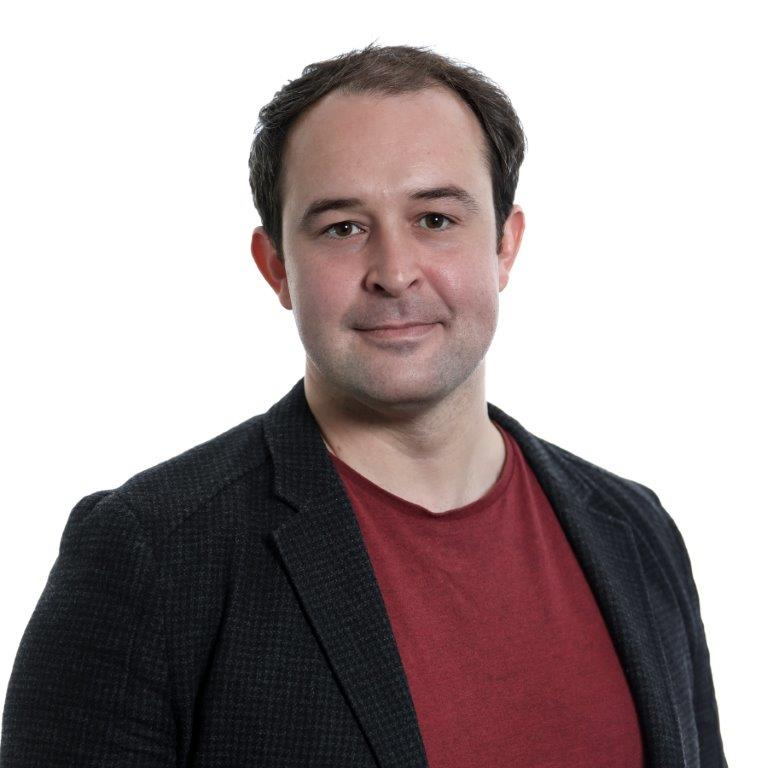
\includegraphics[width=\textwidth]{headshot_roantree.jpg}
			\caption*{\textbf{Lecturer: Prof. Barra Roantree} \\ (Office hours: Wed 12-1pm by appointment)}			
		\end{minipage}
		\hfill
		\pause 
		\begin{minipage}{0.45\textwidth}
			\centering
			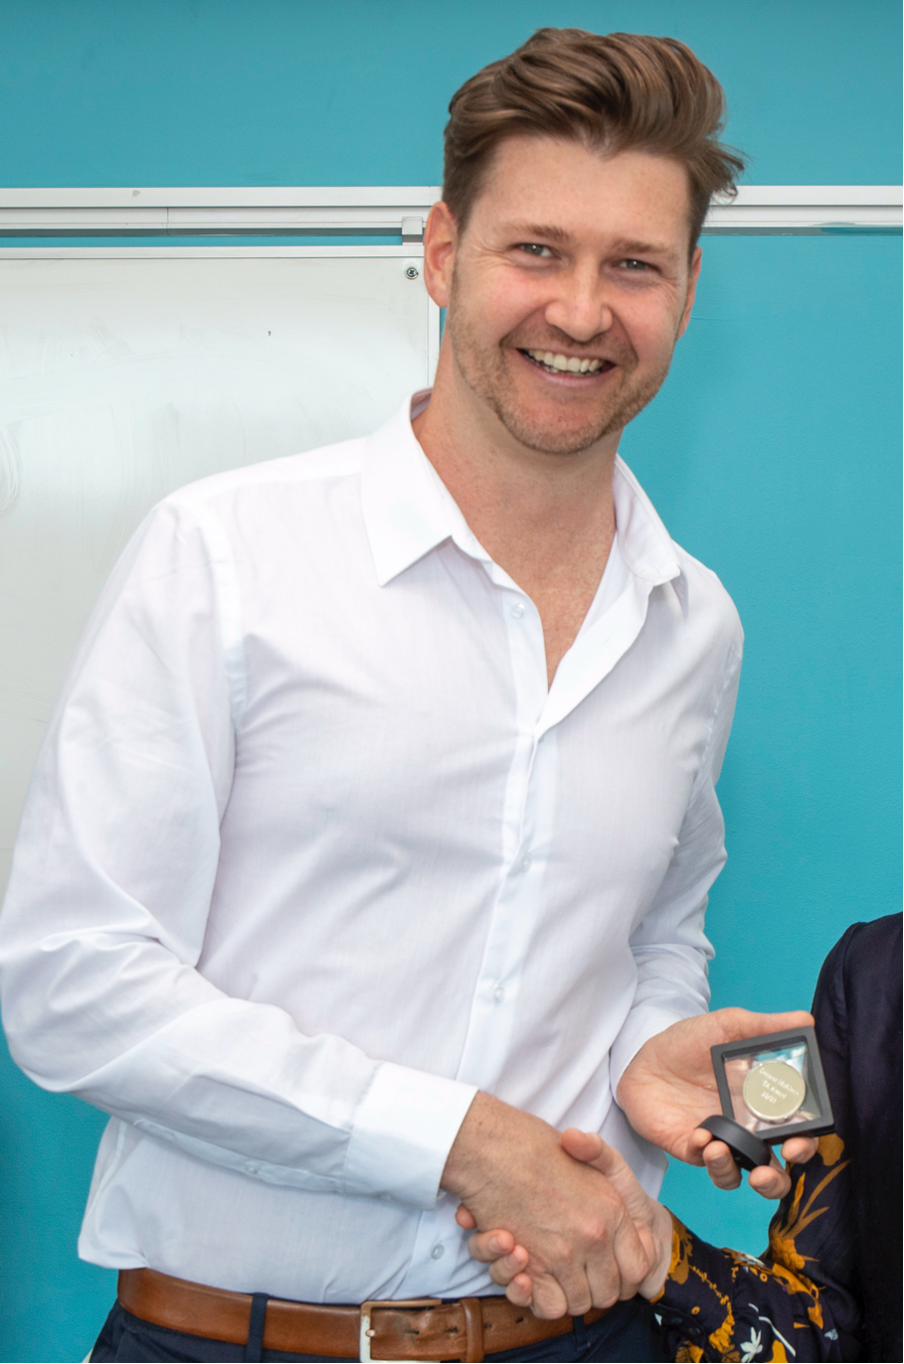
\includegraphics[width=\textwidth, trim=0 250 0 0, clip]{headshot_mcrae.png} % Adjust the trim values as needed
			\caption*{\textbf{TA: Michael McRae} \\ (Office hours: tbc)}
		\end{minipage}
	\end{figure}

\end{frame}

\begin{frame}{Course Preliminaries}
	\framesubtitle{What will you learn in this course?}
	\vspace{0.5cm}
	By the end of the course, should be able to critically assess empirical claims of the sort that are pervasive in life today e.g:
	\pause 
	\begin{figure}
		\centering
		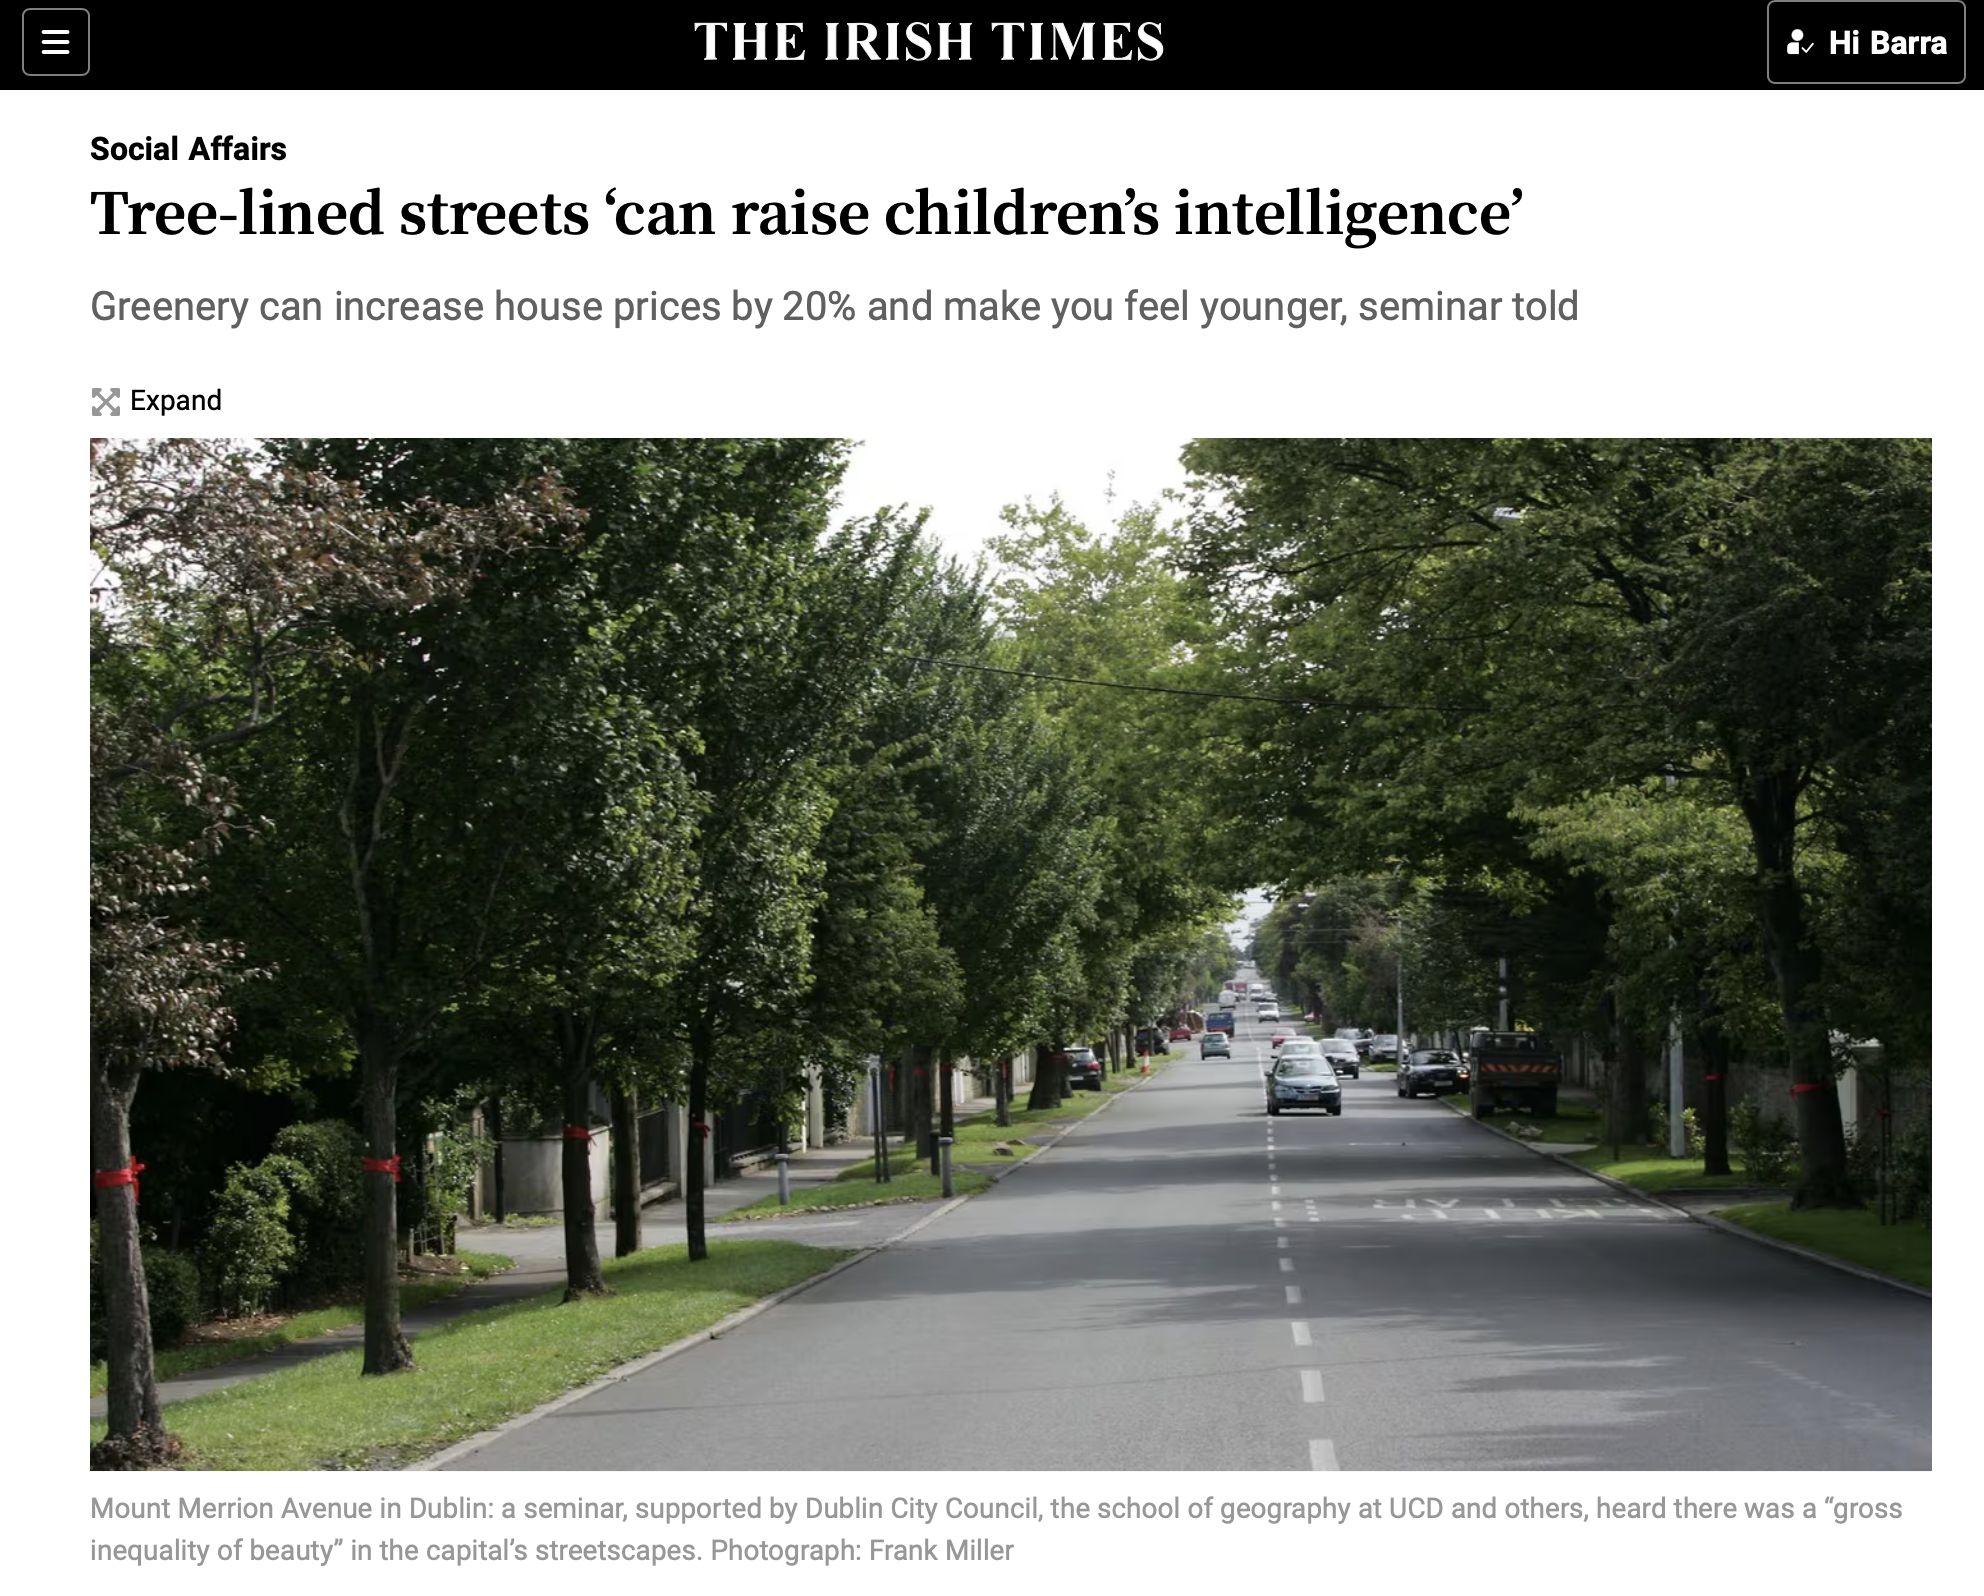
\includegraphics[width=0.6\textwidth, trim=0 0 0 0, clip]{tree-lined-streets.png} % Adjust the trim values as needed
	\end{figure}
	
	\end{frame}
	
\begin{frame}{Course Preliminaries}
	\framesubtitle{What will you learn in this course?}
	\begin{itemize}
		\item Methods for estimating \textit{causal effects} using \textit{observational data} \pause 
		\item Focus on applications: theory is used only as needed to understand the whys of the methods; \pause 
		\item Learn to evaluate the analysis of others: this means you will be able to read/understand empirical economics papers in other econ courses \pause 
		\item Get some hands-on experience with an applied project  
		
	\end{itemize}


\end{frame}

\begin{frame}{Course Preliminaries}
\framesubtitle{Lectures and tutorials}

\textbf{Lectures:}
\begin{itemize}
	\item Wednesday 11am-12pm, Thomas Davis theatre, Arts Building
	\item Friday 12pm-1pm, Regents House (above front arch)
\end{itemize}
\vspace{0.5cm}
\pause 

\textbf{Computer labs:}
\begin{itemize}
	\item Weekly labs \underline{starting week 3} (online intro next week) 
	\item You will learn how to analyse data using software called Stata
	\item Crucial for coursework (worth 30\% of overall grade)
	\item You will be assigned to a group and a time slot by the Department. 
	\item Contact econsec@tcd.ie (\underline{not me or Mike}) if this needs to be changed because of timetable clash (provide details on these)
\end{itemize}
\vspace{0.5cm}
\pause 

Attendance not mandatory \underline{but highly encouraged if you want to pass} 

\end{frame}

\begin{frame}{Course Preliminaries}
	\framesubtitle{Assessment}

\textbf{Courswork (worth 30\%):}
\begin{itemize}
	\item Computer homework (worth 5\%) available next week \& due midday Monday September 23rd
	\item Assignment (worth 25\%) available reading week \& due midday Monday November 18th
	\item Extensions only at the request of your tutor 
\end{itemize}
\vspace{1cm}
\pause 

\textbf{1.5 hours final exam (worth 70\%):}
	\begin{itemize}
		\item Past exam papers available online on Academic Registry webpage
		\item However, structure and content will differ from previous years as module changing a bit this year to better integrate with ECU33092
		
	\end{itemize}
\end{frame}



\begin{frame}{Course Preliminaries}
	\framesubtitle{Textbook and readings}

	\begin{figure}
		\begin{minipage}{0.45\textwidth}
			\centering
			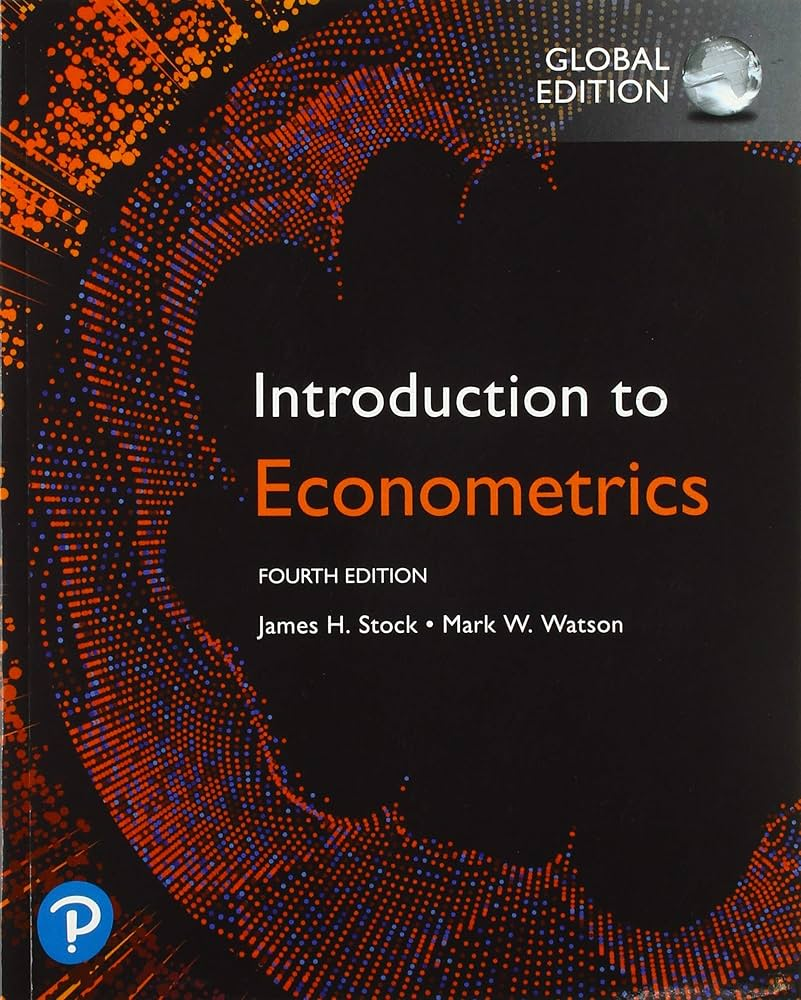
\includegraphics[width=\textwidth]{book_stockwatson.jpg}
		\end{minipage}
		\hfill
		\begin{minipage}{0.45\textwidth}
			\centering
			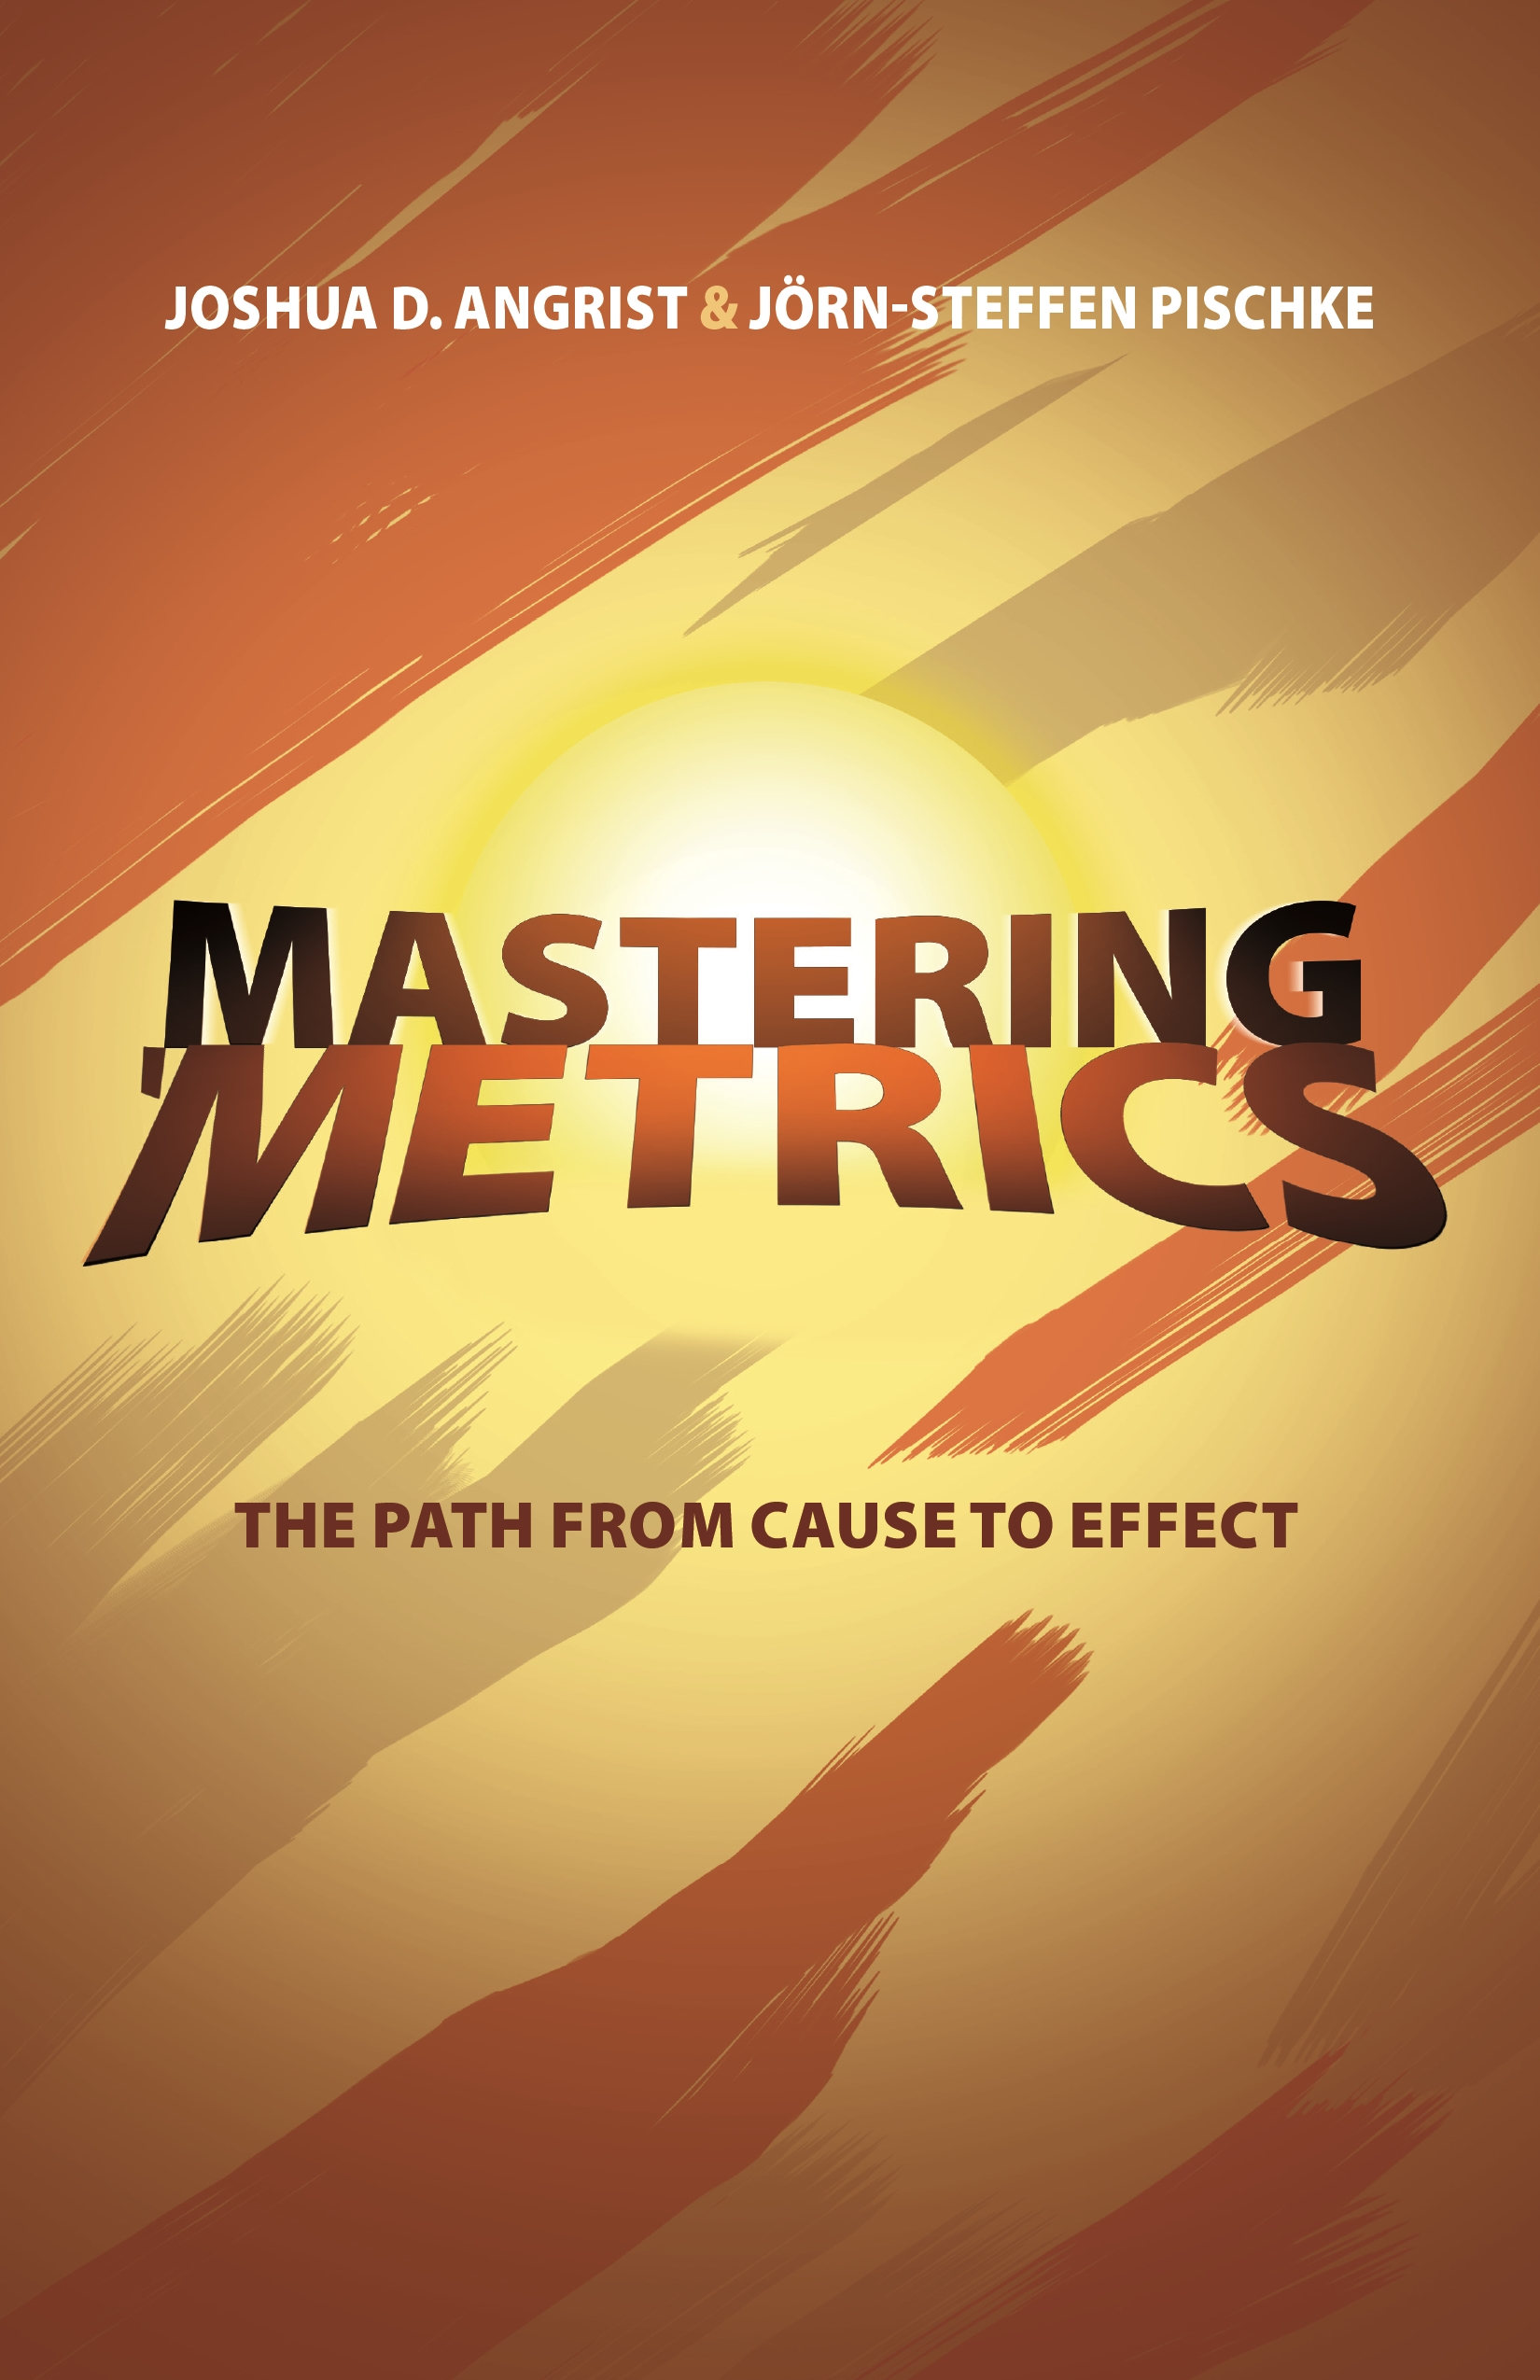
\includegraphics[width=\textwidth]{book_masteringmetrics.jpg}
		\end{minipage}
	\end{figure}


	\vspace{0.5cm}
	Any questions on logistics? 

\end{frame}



\section{What is Econometrics}
\begin{frame}{What is Econometrics?}

\vspace{0.2cm}
$\rightarrow$ The statistical toolkit that economists use to answer economic \uline{questions} with \uline{data}
\vspace{0.25cm} \pause

What types of questions might we be interested in: 
\vspace{0.25cm}

\begin{itemize}
\item<1-> Has economic inequality increased since the 1980s?
	\begin{itemize}
		\item<3-> \textbf{Descriptive Q:} asks about how things are (or were) in reality
	\end{itemize}
\item<1-> How do increases in the minimum wage affect employment? 
	\begin{itemize}
		\item<4-> \textbf{Causal Q:} What would have happened in a counterfactual world?  
	\end{itemize}
\item<1->   What will the unemployment rate be next quarter?
	\begin{itemize}
	\item<5-> \textbf{Forecasting Q:} What will happen in the future?  
\end{itemize}

\end{itemize}
\vspace{0.25cm}

\pause 
\only<6->{
In this module, we will mainly look at descriptive and causal questions (with a strong emphasis on the latter)
}

\end{frame}


\begin{frame}{Answering these types of questions is hard}
\framesubtitle{Descriptive questions}
\pause 
We only observe data for a \textbf{sample}, not the full \textbf{population}
	\begin{itemize}
		\item 
		Example: we want to know how the distribution of earnings in Ireland has changed. But we only observe income for a survey of workers
	\end{itemize}
\vspace{0.25cm}

\pause
\textbf{Best case scenario}: sample \underline{randomly} selected from the population \\
	\begin{itemize}
		\item 
		E.g., the workers in our survey were drawn out of hat with names of all possible workers
		
		\item
		If so, need to account for the fact that by chance the sample might have different characteristics from the population
	\end{itemize}
	\vspace{0.25cm}

\pause
\textbf{Worst case scenario}: sample is \textit{not representative} of the population
	\begin{itemize}
		\item 
		E.g., workers with certain characteristics were more likely to respond to the survey
	\end{itemize}

\end{frame}


\begin{frame}
\centering
\includegraphics[width = 0.7\linewidth]{dewey-defeats-truman}
\begin{itemize}
	\item 
	In 1948, Chicago Tribune writes that Thomas Dewey defeats Harry Truman in the 1948 presidential election, based on survey of voters.
	
	\pause
	\item
	But their survey was conducted by phone. In 1948, only rich people had phones: sample $\neq$ population $\rightarrow$ misleading results!
\end{itemize}

\end{frame}

\begin{frame}
	\textit{Selection bias} referes to settings like Dewey-Truman where the sample is not drawn randomly from the population of interest


	\begin{figure}
		\centering
		\includegraphics[width = 0.6\linewidth]{selection_bias_xkcd.png}
	\end{figure}


\end{frame}


\begin{frame}{Answering these types of questions is hard}
\framesubtitle{Causal questions}
	Answering causal questions often \textit{even harder} than descriptive Qs: why?	
	\pause
	\begin{itemize}
		\item Causal Qs involve both a descriptive component (what are outcomes in reality?) 
		\pause and a \textit{counterfactual} component (how would things have been under a different treatment?)
		
		\pause
		\item e.g: what is the causal effect on your earnings of going to Trinity? 
			\begin{itemize}
				\pause 
				\item Descriptive Q: how much \textit{do} Trinity students earn after graduation?
				% include figure showing trinity student earnings here if can 
				\pause 
				\item Counterfactual Q: how much \textit{would} Trinity students have earned if they went elsewhere?  
			\end{itemize}
	\end{itemize}	
\end{frame}

\begin{frame}{Answering these types of questions is hard}
\framesubtitle{Causal questions}

	Sometimes we can answer causal questions with experiments
	\pause 
	e.g. the causal effect of fertiliser on strawberry yield
	\pause 
	\begin{itemize}
		\item Randomly divide plants into control group where no fertiliser applied and treatment group where fertiliser applied
		\pause 
		\item If the randomisation is properly implemented (i.e. the only difference between treatment \& control group is the treatment), then simple group-difference yields estimate of causal effect  	
	\end{itemize}
	\pause 
	\vspace{0.25cm}

	In many (most?) contexts, this may not be possible \pause 
	\begin{itemize}
		\item e.g. takes too long, costs too much, raises ethical concerns
	\end{itemize}
	\vspace{0.25cm}
	\pause 

	Social scientists need other tools to estimate causal effects

\end{frame}


\section{Course Roadmap}
\begin{frame}{Course Roadmap}
	\subtitle{Where we're going}

	\begin{enumerate}
		\item Causality, poteniatal outcomes, and experiments (MM ch1)
		\item Review of statisitcal tools and inference (MM ch1/SW ch2-3)
		\item Linear regression (SW ch4-5)
		\item Multiple regression (SW ch6-7)
		\item Non-linear regression (SW ch8)
		\item Assessing regression (SW ch8)
		\item Binary outcomes (SW ch11)
		\item Panel data (SW ch10)
	\end{enumerate}

\end{frame}

\section{Data}

\begin{frame}{Data}
\framesubtitle{A short aside on data}
	\pause 
	Econometrics uses data from both experimental \& observational sources \pause 
	\begin{enumerate}
		\item Experimental data: from experiments designed to evaluate a treatment or policy or to investigate a causal effect
		\begin{itemize}
			\item e.g. Preparing for Life https://www.preparingforlife.ie/ 
		\end{itemize}
		\pause 
		
		\item Observational data: collected in surveys or administrative records
		\begin{itemize}
			\item e.g. EU Survey of Income and Living Conditions (EU-SILC)
			\item e.g. UK HM Revenue and Customs Data Lab 
		\end{itemize}	
	\end{enumerate}
\end{frame}

\begin{frame}{Data}
\framesubtitle{From either experimental or observational sources, 3 main types of data:}
	 \pause 
	\begin{enumerate}
		\item Cross-sectional: multiple entities observed at a single time period \pause  
		\item Time series: single entity observed at multiple time points \pause 
		\item Panel/longitudinal: multiple entities, with each observed at two or more time periods
	\end{enumerate}

\end{frame}

\begin{frame}{Data}
\framesubtitle{Cross-sectional data}
	\begin{figure}
		\centering
		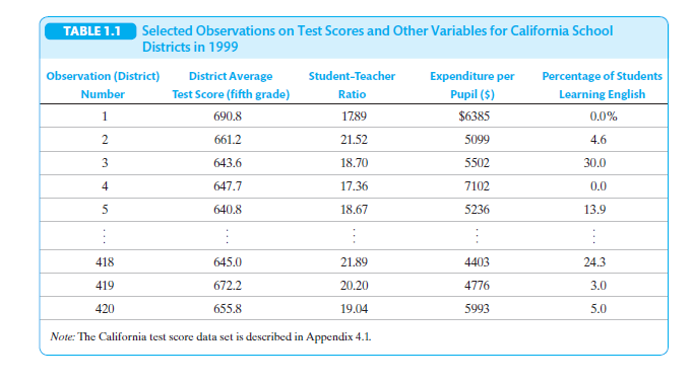
\includegraphics[width = 0.9\linewidth]{xsection_data.png}
	\end{figure}
\end{frame}

\begin{frame}{Data}
\framesubtitle{Time series data}
	\begin{figure}
		\centering
		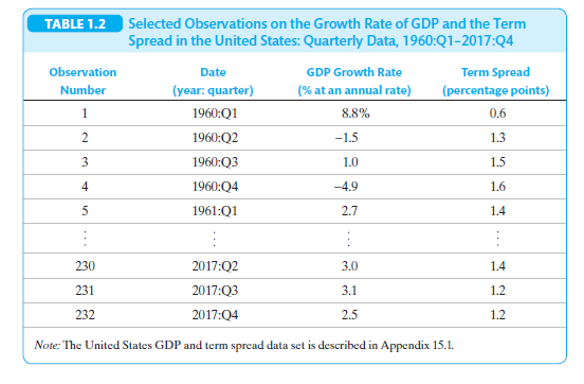
\includegraphics[width = 0.9\linewidth]{ts_data.png}
	\end{figure}
\end{frame}

\begin{frame}{Data}
	\framesubtitle{Panel/longitudinal data}
		\begin{figure}
			\centering
			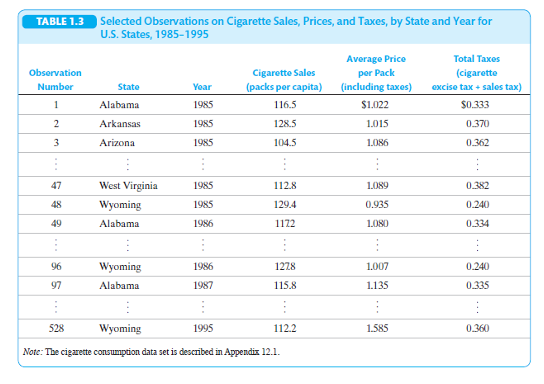
\includegraphics[width = 0.9\linewidth]{panel_data.png}
		\end{figure}
	\end{frame}

\begin{frame}{And finally: the Student Economic Review}


	\begin{figure}
		\centering
		
\includegraphics[width=0.4\textwidth]{ser_logo.png}
	\end{figure}
	\begin{itemize}
		\item Founded in 1987, the Student Economic Review (SER) is one of the oldest undergraduate journals in the world
		\item Committee chosen by academic staff from JS economics students
		\item Email will be going out shortly: think about applying!
		\item See https://www.tcd.ie/Economics/SER/ 
	\end{itemize}


\end{frame}

\begin{frame}
	\centering
	\Huge{See you on Friday (midday in Regents House)}
\end{frame}


\end{document}
}
